\subsection{\'Ordenes: Google vs PageRank vs In-Deg}
\label{subsec:exp2}
\begin{LaTeXdescription}
    \item[Objetivo] Analizar el orden obtenido respecto de otros \'ordenes
        disponibles. ¿Es igual? ¿Hay coincidencias? ¿Cu\'antas? ¿Tienen sentido?

    \item[Proposici\'on] Cualitativamente hablando, ¿c\'omo es el orden obtenido
        por PageRank? ¿Bueno? ¿Malo?. Obviamente que estas categorizacones son
        intr\'insecas a la realidad: s\'olo nosotros podemos decir que al
        realizar una b\'usqueda web, los resultados vinieron en un orden
        correcto o deseable (es decir, lo que se buscaba en las primeras
        posiciones).  Utilizar nuestro criterio personal para hablar de la
        calidad del orden obtenido no ser\'ia muy correcto, ya que cualquier
        otra persona con criterios distintos podr\'ia disentir y ninguno de los
        criterios ser\'ia \textit{a priori} m\'as correcto que el
        otro\footnote{Se podr\'ia ver muestralmente que opina la gente de
        distintos \'ambitos, pero esto escapa al objeto de estudio de este
        trabajo.}. Pero lo que si podemos hacer es comparar el resultado
        obtenido con otros resultados disponibles, de los cuales proponemos
        In-Deg (que se basa en el grafo de conectividad) y los resultados de un
        search engine: Google.

    \item[M\'etodo de Experimentaci\'on] Utilizamos la misma instancia que en el
        experimento anterior. Sobre esta instancia s\'olo nos falta calcular el
        orden In-Deg (el cual no es otra cosa que ordenar a los nodos en orden
        descendiente seg\'un su grado de entrada, es decir seg\'un la cantidad
        de ejes que los apuntan). Luego utilizamos el orden provisto por Google
        en la b\'usqueda inicial m\'as los \'ordenes obtenidos en el experimento
        previo.

    \item[Resultados, an\'alisis y discusi\'on]
\end{LaTeXdescription}

\begin{table}[hb]
    \centering
    \caption{\'Ordenes comparativos entre los Resultados Google, PageRank e
        In-Deg}
        \label{tbl:google_pagerank_vs_indeg_siteubaar} 
    \setlength{\tabcolsep}{3pt}
    \begin{tabular}{|l|l|l|}
        \hline\hline
        Google & PageRank & In-Deg\\
        \hline
        www.derecho.uba.ar & videos.agro.uba.ar& videos.agro.uba.ar\\
        orga2.exp.dc.uba.ar & www.uba.ar& www.uba.ar\\
        www.agro.uba.ar & www.agro.uba.ar& www.agro.uba.ar\\
        www.ffyb.uba.ar & www.agro.uba.ar/cursos& www.agro.uba.ar/ced\\
        www.uba.ar & www.agro.uba.ar/ced& www.agro.uba.ar/cursos \\
        www.fvet.uba.ar & www.fvet.uba.ar& www.fvet.uba.ar\\
        videos.agro.uba.ar & www.ffyb.uba.ar& www.ffyb.uba.ar\\
        iigg.sociales.uba.ar& www.derecho.uba.ar& www.derecho.com.ar\\
        www.agro.uba.ar/cursos & iigg.sociales.uba.ar& iigg.sociales.uba.ar\\
        www.agro.uba.ar/ced & orga2.exp.dc.uba.ar& orga2.exp.dc.uba.ar\\
        \hline\hline
    \end{tabular}
\end{table}

\par Dado que los resultados obtenidos en
\ref{tbl:google_pagerank_vs_indeg_siteubaar} dieron resultados similares en
cuanto a In-Deg vs PageRank, e intuyendo que esto no tiene que ser siempre
as\'i, realizamos un nuevo experimento. Esta vez buscamos en
wikipedia\cite{wikipedia} distintos t\'erminos relacionados con los temas vistos
en la materia. Sobre estas p\'aginas, calculamos los \'ordenes de PageRank e
In-Deg, para luego compararlos en el cuadro
\ref{tbl:pagerank_vs_indeg_wikipedia} . Nuevamente, In-Deg y PageRank dieron
resultados muy similares. Sin embargo, podemos observar que quedan primeros en
el ranking terminos mas \texttt{generales o abarcativos} y a medida que avanza
el ranking se encuentran términos mas particulares. Para evidenciar la
diferencia entre los algoritmos de In-Deg y PageRank decidimos alterar
explicitamente el grafo de conectividad, agregando aristas desde los últimos 5
resultados hacia el último en el ranking. Esto deberia aumentar drásticamente el
rankeo del ultimo elemento en In-Deg, no asi en Pagerank, los resultados de este
último experimento pueden verse en el cuadro
\ref{tbl:pagerank_vs_indeg_wikipedia_modificado}. Lamentablemente no vemos los
resultados tan drásticos que esperabamos entre In-Deg y PageRank, puede deberse
a que las instancias de prueba son muy chicas, o a que el experimento de agregar
5 aristas, incremento el rankeo de pagerank mas de lo que esperabamos. Por
último, vemos que en el último experimento se acentúa el orden
\texttt{abarcativo} de los resultados respecto al dominio de los elementos.

\begin{figure}[H]
    \centering
    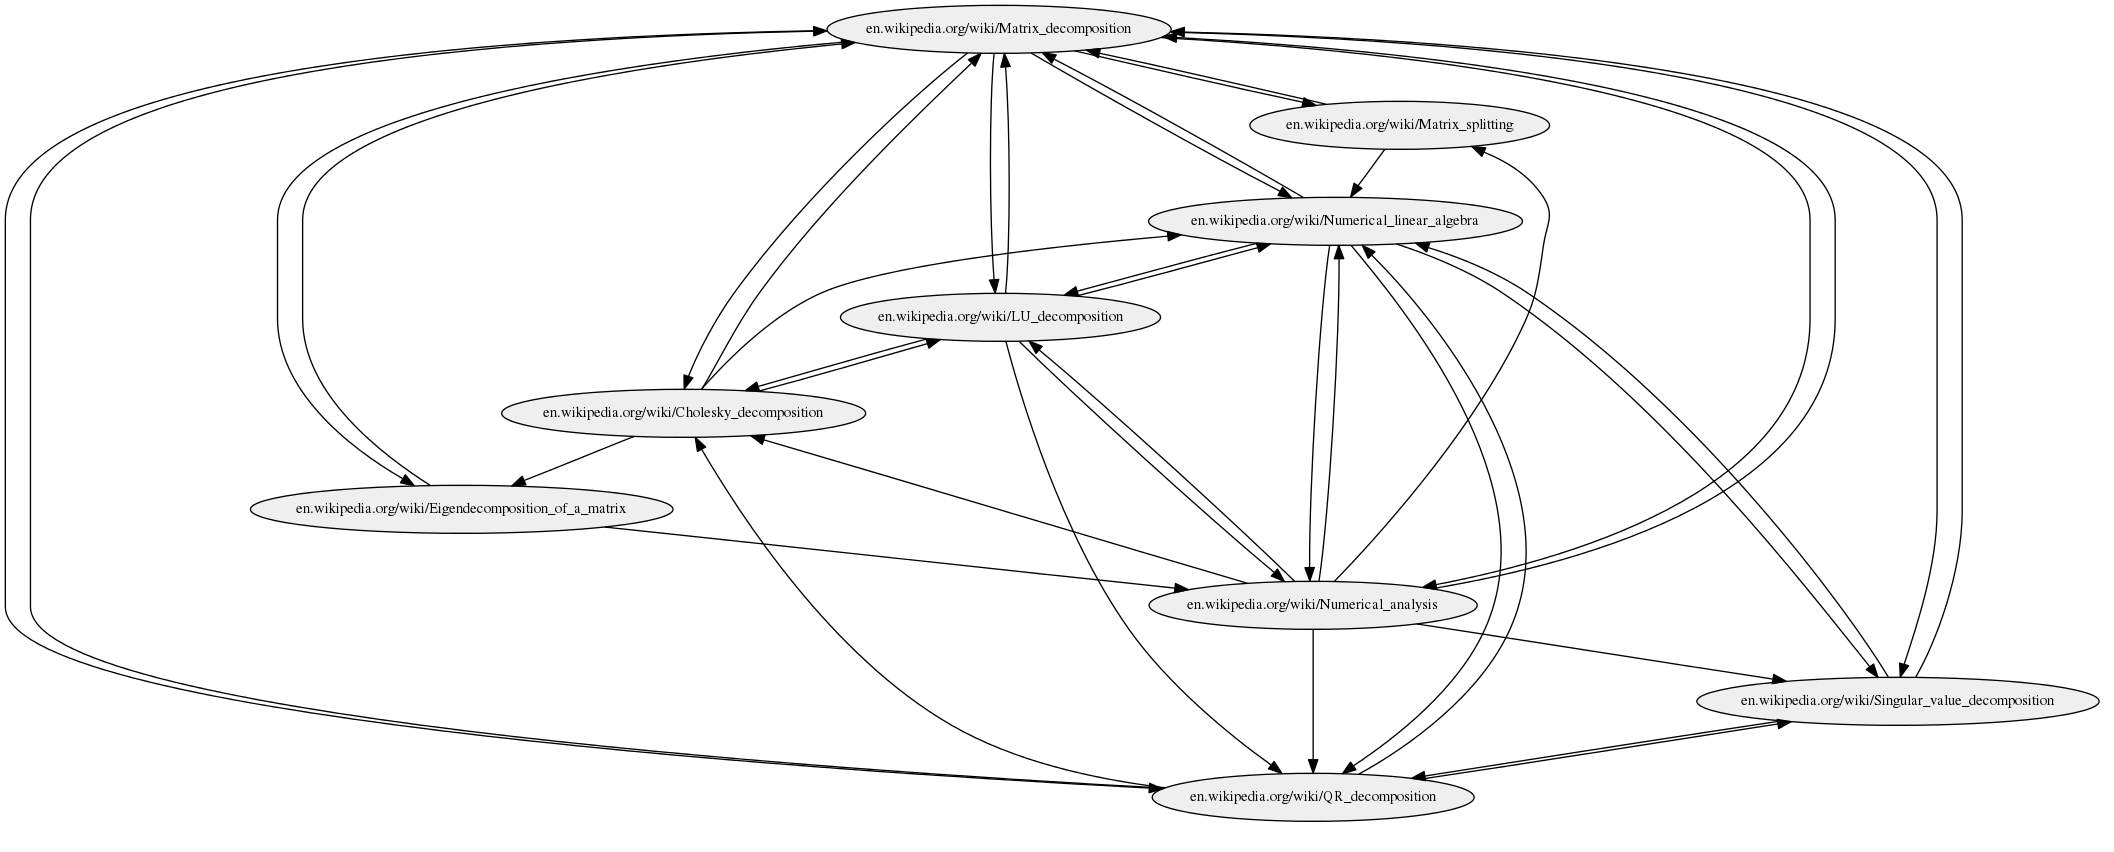
\includegraphics[angle=90,height=\textheight]{exp2_conn_graph_metodos.png}
    \caption{Grafo de conectividad de p\'aginas de Wikipedia relacionadas con
        m\'etodos num\'ericos}
    \label{wiki_graph}
\end{figure}

\begin{table}[h]
    \centering
    \caption{\'Ordenes comparativos entre PageRank e In-Deg para Wikipedia}
    \label{tbl:pagerank_vs_indeg_wikipedia} 
    \setlength{\tabcolsep}{3pt}
    \begin{tabular}{|l|l|}
        \hline\hline
        PageRank & In-Deg\\
        \hline
        Matrix\_decomposition& Matrix\_decomposition\\
        Numerical\_linear\_algebra& Numerical\_linear\_algebra\\
        QR\_decomposition& QR\_decomposition\\
        Numerical\_analysis& Singular\_value\_decomposition\\
        Singular\_value\_decomposition& Numerical\_analysis\\
        LU\_decomposition& LU\_decomposition\\
        Cholesky\_decomposition& Cholesky\_decomposition\\
        Eigendecomposition\_of\_a\_matrix& Matrix\_splitting\\
        Matrix\_splitting& Eigendecomposition\_of\_a\_matrix\\
        \hline\hline
    \end{tabular}
\end{table}

\begin{table}[h]
    \centering
    \caption{\'Ordenes comparativos entre PageRank e In-Deg para Wikipedia con grafo modificado explícitamente}
    \label{tbl:pagerank_vs_indeg_wikipedia_modificado}
    \setlength{\tabcolsep}{3pt}
    \begin{tabular}{|l|l|}
        \hline\hline
        Pagerank & Indeg\\
        \hline
        Matrix\_decomposition & Matrix\_decomposition\\
        Numerical\_linear\_algebra & Numerical\_linear\_algebra\\
        Numerical\_analysis & Eigendecomposition\_of\_a\_matrix  \\
        Eigendecomposition\_of\_a\_matrix & QR\_decomposition\\
        QR\_decomposition & Singular\_value\_decomposition\\
        Singular\_value\_decomposition & Numerical\_analysis  \\
        LU\_decomposition & LU\_decomposition\\
        Cholesky\_decomposition & Cholesky\_decomposition  \\
        Matrix\_splitting & Matrix\_splitting\\
        \hline\hline
    \end{tabular}
\end{table}
